\documentclass[main.tex]{subfiles}

\begin{document}

\chapter{Preassembly}\label{chapter:preassembly}

% Assembly are based on :
% - reads, reads contains error, this error isn't rept
% - overlaps
Assembly are based on reads if your reads are bad your assembly are bad you can't reconstruct the book if the crazy monk give to you only a sequence of letter, with an half of them is an error. Correction of read with a mix of sequencing technology or not, can help you to get better read but actualy tools have an important cost in term of computation time and memory usage, moreover it's hard to differentiate natural mutation to sequencing error and sometimes natural interesting mutation was consider as error and corrected.

With long-read, reads contain many error and these errors are not uniformly distributed in read along the read \cite{blog_post_error_repartition}, these errors make it more difficult to search overlaps between reads and current heuristics can further improve their results on real data \cite{ovl_bench}.
And in overlap found by this tools not all of them are useful to each downstream analysis, for example \miniasm keep only end to end overlap and \canu two longest end to end overlap for each read (see \ref{chapter:sota} for more details).

Our paper "\yacrd and \fpa: upstream tools for long-read genome assembly" focus on two tools \yacrd (for Yet Another Chimeric Read Detector) and \fpa (for Filter Pairwise Alignment). \yacrd focus on detection and elimination of very poor quality region, \fpa focus on filtering of overlap.

In \cite{ovl_bench} \citeauthor{ovl_bench} compare state of the art of overlapper on simulated dataset and on real dataset, a drop in the accuracy and recall of these algorithms can be observed between real and simulated data \ref{preassembly:tab:ovl_result}.

\begin{table}[ht]
    \centering
    \begin{tabular}{l|rr|rr}
                & \multicolumn{2}{c}{Pacbio}                & \multicolumn{2}{c}{Nanopore}              \\ 
                & Simulated           & Real                & Simulated         & Real                  \\ \hline
    Sensibility & 88.9$^m$ - 92.4$^d$ & 59.6$^m$ - 83.8$^d$ & 90.4$^g$ - 95.2$^b$ & 88.9$^b$ - 92.9$^d$ \\
    Precision   & 81.9$^b$ - 96.5$^g$ & 79.8$^h$ - 96.5$^b$ & 75.1$^b$ - 99$^m$   & 73$^b$ - 95.4$^m$   \\
    \end{tabular}
    \caption{\textsuperscript{m}\toolsname{Minimap}, \textsuperscript{d}\toolsname{Daligner}, \textsuperscript{g}\toolsname{GraphMap}, \textsuperscript{b}\toolsname{BLASR}, \textsuperscript{h}\mhap}
    \label{preassembly:tab:ovl_result}
\end{table}

In the blog post "State-of-the-art long reads overlapper-compare" \footnote{\url{https://blog.pierre.marijon.fr/long-reads-overlapper-compare/}} we take same data as \cite{ovl_bench} but we didn't search if overlapper found good and wrong overlap we search if they found the same overlap. There were differences large enough to justify the idea of creating an overlap reconciler a prototype was created by a master student. 
This blog post was present as poster during JOBIM (Journée Ouverte de Bioinformatique \& Mathematique) 2018.


In this chapter we present to you this two work.


\subfile{paper/yacrd_fpa.tex}
%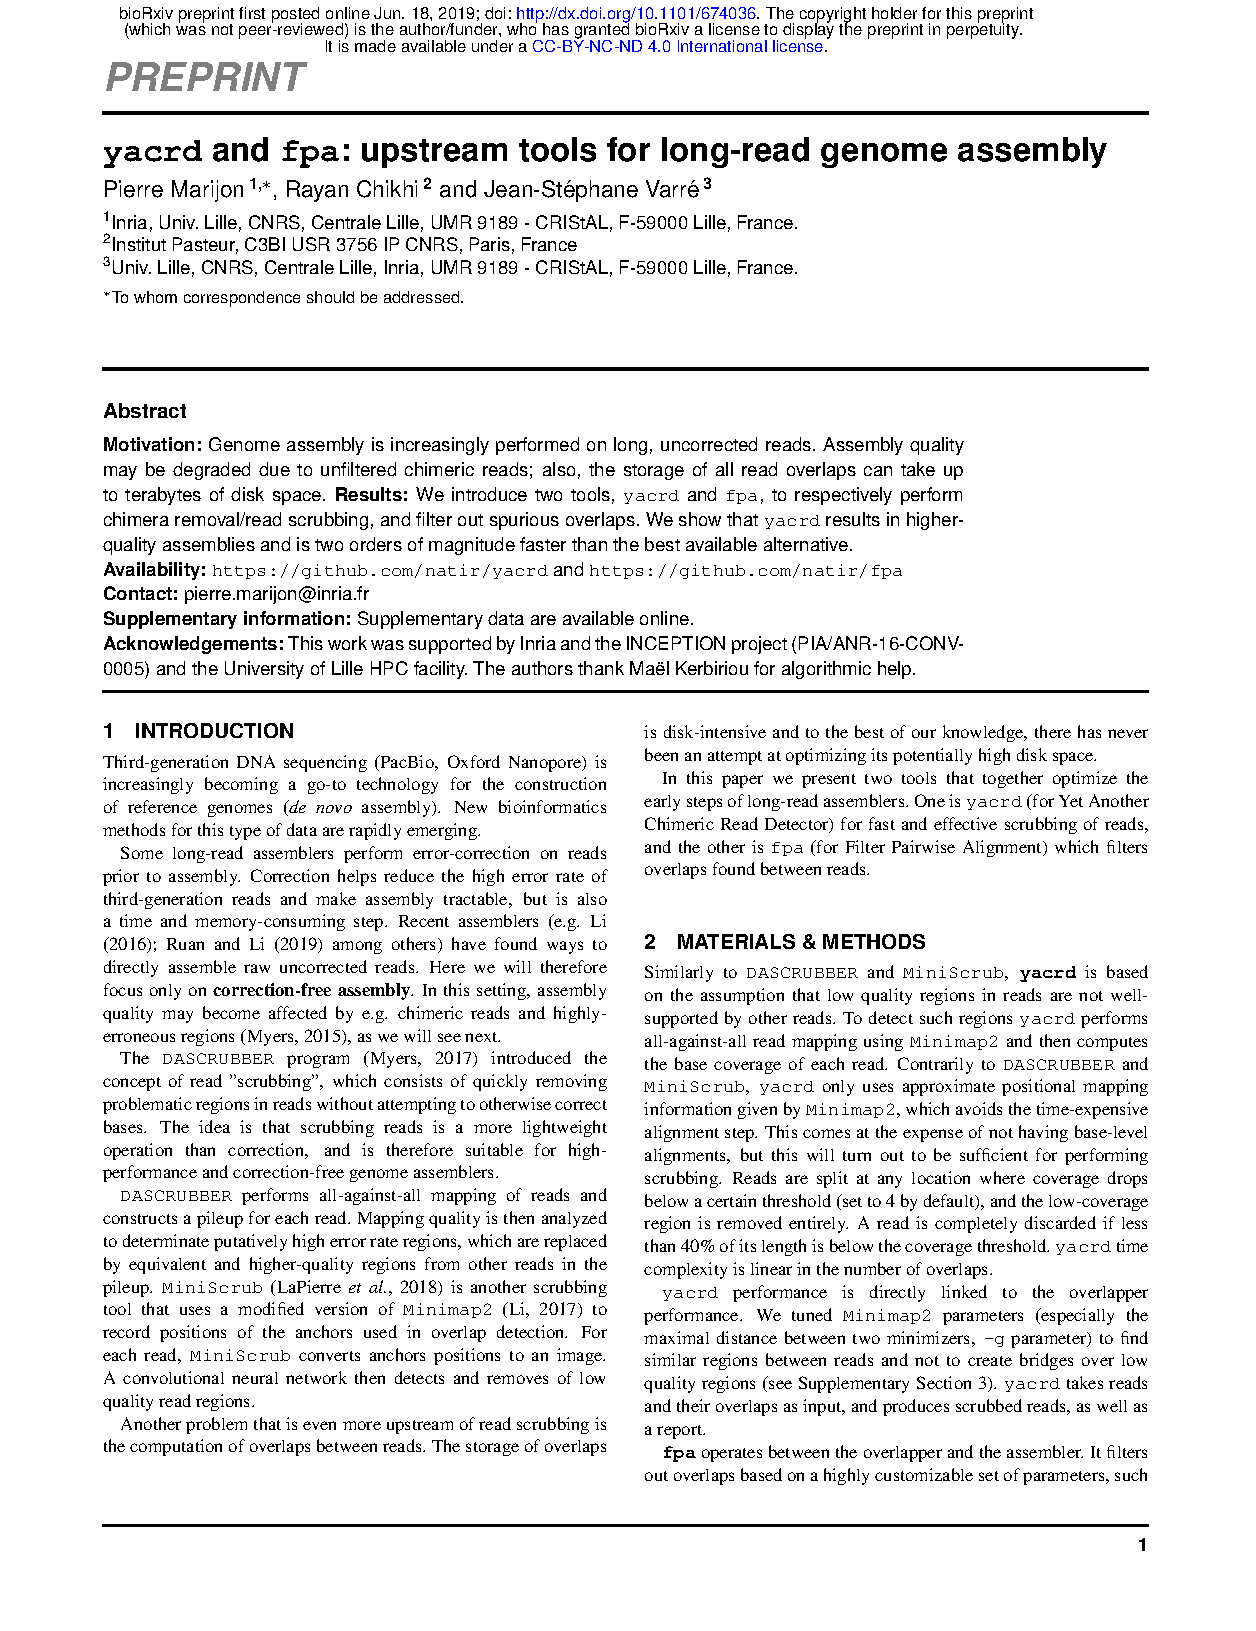
\includepdf[pages=-]{paper/yacrd_fpa.pdf}


\section{Overlapping consensus}\label{section:preassembly:ovl_consensus}

\onlyinsubfile{
\bibliographystyle{plainnat}
\bibliography{main}
\addcontentsline{toc}{chapter}{Bibliography}
}

\end{document}